\section{Base Performance}

Of course before we look into some potentially beneficial alterations we could make to Raft, we must examine the base algorithms ability to scale. Using a simple implementation of Raft with the \textit{hashicorp/raft} library, we started up clusters of varying sizes, and ran 100 successive write then read operations, and timed how long it took to complete \cite{HashicorpRaft}.

\begin{figure}[h]
\centering
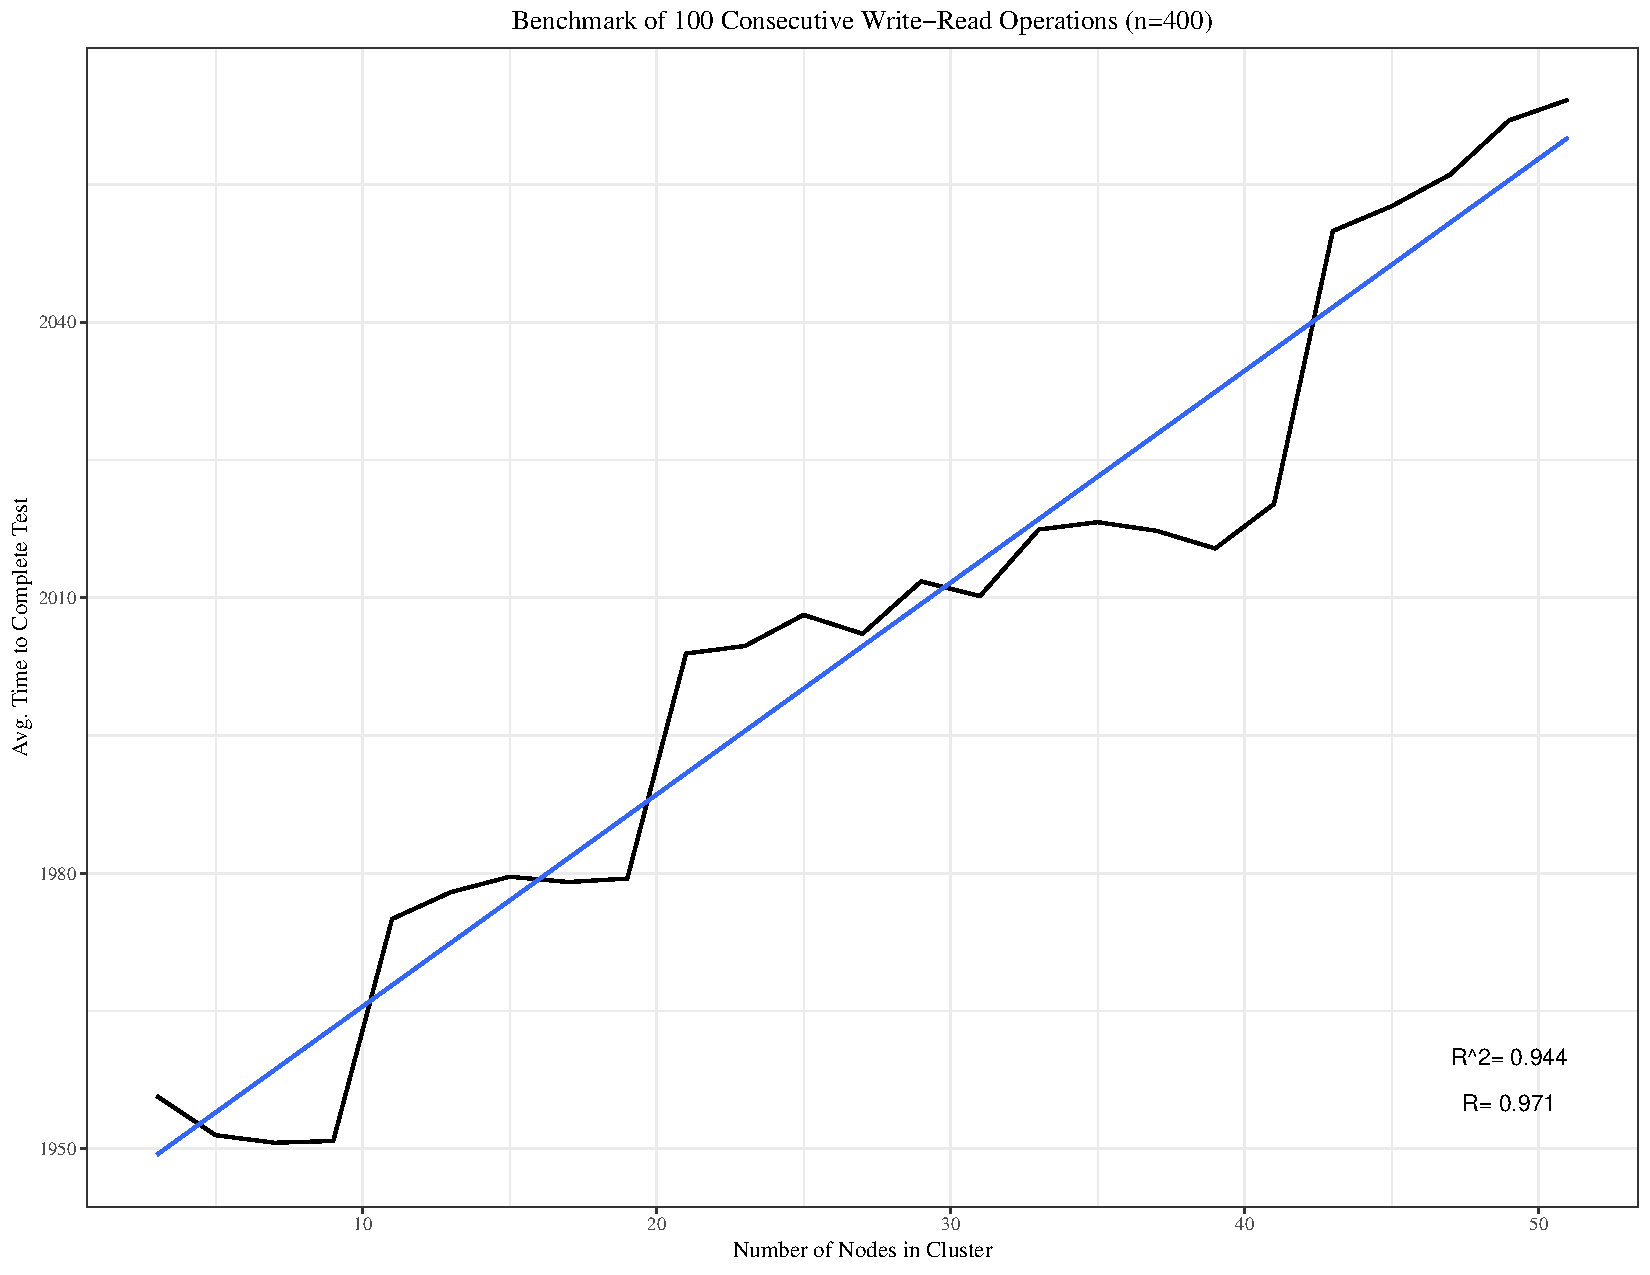
\includegraphics[width=0.5\textwidth]{benchmark.pdf}
\end{figure}

As we see in this test, as we increase the number of nodes in a cluster, even without any extra difficulties like delays or node failures, consensus becomes harder to achieve. After this observation we can start to investigate improving the rate at which the time it takes to reach distributed agreement.